\documentclass{sprawozdanie-agh}

\usepackage[utf8]{inputenc}
\usepackage{listings}
\usepackage{tikz}
\usepackage{xcolor}
\usepackage{graphicx}
\usepackage{caption}
\usepackage{lipsum}
\usepackage{wrapfig}
\usepackage{subcaption}
\usepackage{accsupp}
\usepackage{array}
\usepackage{multirow}
\usepackage{amsmath}
\usepackage{siunitx}    
\usepackage{pgfplots}
\usepackage{pgfplotstable}

\graphicspath{ {./images/} }
\pgfplotsset{compat = newest}

\usetikzlibrary{angles,quotes}
\makeatletter

\begin{document}

\przedmiot{Metody Obliczeniowe w Nauce i Technice}
\tytul{Laboratorium 1}
\podtytul{Analiza błędów}
\kierunek{Informatyka}
\autor{Wojciech Michaluk, Kyrylo Iakymenko}
\data{Kraków, 1 marca 2024}

\stronatytulowa{}

\section{Wprowadzenie}

\quad Podczas tego laboratorium zrealizujemy 2 zadania, na podstawie których będziemy przeprowadzać analizę błędów - jest ich bowiem wiele rodzajów. 

W zadaniu pierwszym skupimy się na błędach obliczeniowych, numerycznych i~błędach metody. Przedstawimy je na przykładzie obliczania pochodnej wybranej funkcji w~punkcie, przybliżając ją za pomocą ilorazu różnicowego i~wykonamy obliczenia dla różnych wartości kroku. Skorzystamy z~odpowiednich zależności, aby obliczyć błędy i~zaprezentujemy je na wspólnym wykresie. 

Z kolei zadanie drugie polega na obliczania kolejnych wyrazów ciągu rekurencyjnego zdefiniowanego równaniem różnicowym, przyjmując różne reprezentacje liczb zmiennoprzecinkowych. Dla każdej z~nich przeanalizujemy otrzymane wartości wyrazów ciągu i~porównamy z~teoretycznymi, następnie przedstawimy odpowiednio błędy względne w~każdej z~reprezentacji.

\section{Zadanie 1}

\subsection{Opis zadania}

\quad W~zadaniu należy obliczyć wartość pochodnej funkcji, używając najpierw wzoru na różnicę prawostronną:

\begin{equation}
	f'(x) \approx \frac{f(x+h)-f(x)}{h},
	\label{zad1:eqn1}
\end{equation}
a~następnie używając wzoru różnic centralnych, czyli

\begin{equation}
	f'(x) \approx \frac{f(x+h)-f(x-h)}{2h}.
	\label{zad1:eqn2}
\end{equation}
Rozważaną funkcją jest $tan(x)$ w~punkcie $x=1$, natomiast przyjmowane wartości $h$~wynoszą $10^{-k}, k=0,1,...,16$.

Kolejnym etapem jest wyznaczenie błędu metody, błędu numerycznego i~błędu obliczenowego w~zależności od $h$~oraz odpowiednie ich przedstawienie na wspólnym wykresie i~wyciągnięcie wniosków.

Do obliczenia wspomnianych błędów pomocne będzie skorzystanie z~tożsamości 

\begin{equation}
	tan'(x)=1+tan^2(x),
	\label{zad1:eqn3} 
\end{equation}
która pozwala wyznaczyć rzeczywistą wartość pochodnej.

\subsection{Podejście pierwsze - różnica prawostronna}

\quad W~tym przypadku zachodzi zależność \footnote{Wzór zaczerpnięty z~\cite{teams_materials}.}

\begin{equation}
	E(h) \le \frac{Mh}{2}+\frac{2\epsilon}{h},
	\label{zad1:eqn4}
\end{equation}
gdzie:

\begin{itemize}
	\item błąd metody, zwany także błędem obcięcia (\emph{truncation error}) jest wyrażony wzorem $\frac{Mh}{2}$, natomiast $M$~to przybliżona wartość drugiej pochodnej rozważanej funkcji w~punkcie $x=1$. Tutaj $M \approx 10.669859$.
	\item błąd numeryczny (\emph{rounding error}) to $\frac{2\epsilon}{h}$, przy czym $\epsilon$~oznacza precyzję przedstawienia liczby w~przyjętej reprezentacji zmiennoprzecinkowej, tzw. $\epsilon_{mach}$ - najmniejsza liczba, dla której (jeszcze) jest spełniony warunek $1+\epsilon > 1$, biorąc pod uwagę reprezentację zmiennoprzecinkową wyniku operacji $1+\epsilon$. W tym zadaniu używamy reprezentacji float64, $\epsilon \approx 2.220446 \cdot 10^{-16}$.
	\item błąd obliczeniowy $E(h)$ (\emph{computational error}) jest to różnica między uzyskanym wynikiem a~wartością obliczoną ze wzoru~(\ref{zad1:eqn3}).
\end{itemize}
Przedstawiamy wykresy wartości bezwzględnych błędów na wspólnym wykresie, przy czym na obu osiach użyto skali logarytmicznej.

\begin{figure}[h!]
	\centering{
		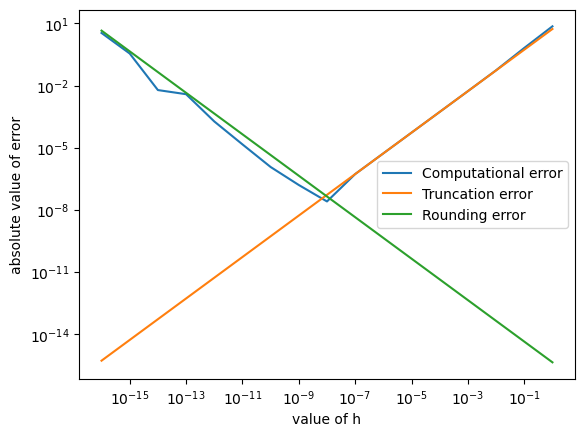
\includegraphics[width=0.67\textwidth]{img/deriv_right_err.png}
	}
	\caption{Wykres wspólny wartości bezwględnych błędów - różnica prawostronna}
	\label{zad1:graph1}
\end{figure}

Zauważmy, że wykresy błędów zachowują się zgodnie z~przewidywaniami opartymi na zależności~(\ref{zad1:eqn4}). Ponadto można stwierdzić, że wykres błędu obliczeniowego ma w~pewnym punkcie minimum - mianowicie w~$10^{-8}$, natomiast należy wziąć poprawkę na fakt, że punkty wykresu zostały połączone prostymi liniami, aby zwiększyć czytelność. Poniżej przedstawiamy obliczenia prowadzące do wyznaczenia dokładnej wartości $h_{min}$, dla której prawa strona nierówności~(\ref{zad1:eqn4}) przyjmuje najmniejszą wartość. Mamy zatem

\begin{align}
	\frac{\partial{(\frac{Mh}{2}+\frac{2\epsilon}{h}})}{\partial{h}} &= 0 \\
	\frac{M}{2}-\frac{2\epsilon}{h^2} &= 0 \\
	h^2 &= \frac{4\epsilon}{M} \\ 
	h_{min} = h &= 2\sqrt{\frac{\epsilon}{M}}
\end{align}
Podstawiając wartości $\epsilon$~i~$M$, uzyskujemy $h_{min} \approx 9.123695 \cdot 10^{-9}$.

Przejdźmy zatem do obliczenia wartości bezwględnej błędu względnego (obliczeniowego) w~punkcie~$h_{min}$. Wyliczamy ją ze wzoru $\left| \frac{E(h_{min})}{tan'(1)} \right|$ i~otrzymujemy 
$$
\left| \frac{E(h_{min})}{tan'(1)} \right| \approx 5.33866349 \cdot 10^{-9}
$$.

\newpage

\subsection{Podejście drugie - różnica centralna}

Przy tym podejściu zachodzi zależność \footnote{Wzór zaczerpnięty z~\cite{teams_materials}.}

\begin{equation}
	E(h) \le \frac{Mh^2}{6}+\frac{\epsilon}{h},
	\label{zad1:eqn9}
\end{equation}
gdzie:

\begin{itemize}
	\item błąd metody jest wyrażony wzorem $\frac{Mh^2}{6}$ i~w~tym przypadku $M \approx 56.7029999$, 
	\item błąd numeryczny to $\frac{\epsilon}{h}$ ($\epsilon$ ma taką samą wartość jak w~pierwszym podejściu),
	\item błąd obliczeniowy $E(h)$ jest, tak jak poprzednio, różnicą między uzyskanym wynikiem a~wartością obliczoną ze wzoru~(\ref{zad1:eqn3}).
\end{itemize}
Przedstawiamy wykresy wartości bezwzględnych błędów na wspólnym wykresie, przy czym na obu osiach użyto skali logarytmicznej.

\begin{figure}[h!]
	\centering{
		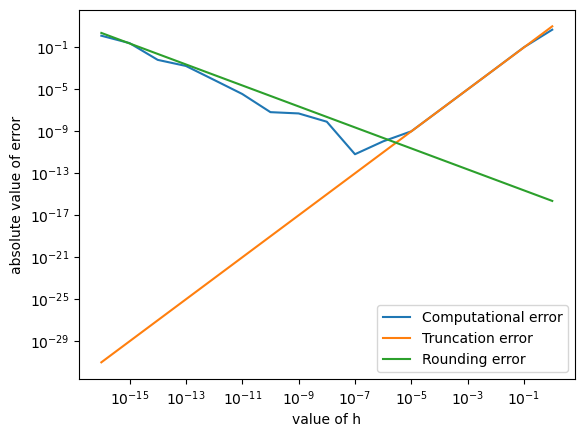
\includegraphics[width=0.67\textwidth]{img/deriv_central_err.png}
	}
	\caption{Wykres wspólny wartości bezwględnych błędów - różnica centralna}
	\label{zad1:graph2}
\end{figure}

Podobnie jak w~pierwszym podejściu, tutaj także wykresy zachowują się zgodnie z~przewidywaniami wedle zależności~(\ref{zad1:eqn9}) oraz wykres błędu obliczeniowego ma w~pewnym punkcie minimum, które tym razem graficznie przypada w~$10^{-7}$. Poniżej przedstawiamy obliczenia prowadzące do wyznaczenia dokładnej wartości $h_{min}$, dla której prawa strona nierówności~(\ref{zad1:eqn9}) przyjmuje najmniejszą wartość. Mamy zatem

\begin{align}
	\frac{\partial{(\frac{Mh^2}{6}+\frac{\epsilon}{h}})}{\partial{h}} &= 0 \\
	\frac{Mh}{3}-\frac{\epsilon}{h^2} &= 0 \\
	h^3 &= \frac{3\epsilon}{M} \\ 
	h_{min} = h &= \sqrt[3]{\frac{3\epsilon}{M}}
\end{align}
Podstawiając wartości $\epsilon$~i~$M$, uzyskujemy $h_{min} \approx 2.273274 \cdot 10^{-6}$.

Możemy teraz obliczyć wartość bezwględną błędu względnego w~wyznaczonym punkcie~$h_{min}$. Postępując analogicznie, w~tym przypadku wynosi ona $\approx 2.53340126 \cdot 10^{-11}$.

\newpage


\section{Zadanie 2}

\subsection{Opis zadania}

\quad Celem tego ćwiczenia jest zrozumienie sposobu rozwiązywania równań różnicowych przy użyciu iteracji oraz analiza wpływu precyzji obliczeń na wyniki.
Rozważmy następujące równanie różnicowe:
\begin{align*}
        x_{k+1} = 2.25x_k - 0.5x_{k-1},\\
        \textrm{gdzie } x_0 = \frac{1}{3}, x_1 = \frac{1}{12}.
\end{align*}

Zadanie polega na wygenerowaniu pierwszych $n$ wyrazów tego ciągu oraz analizie zachowania się ciągu w zależności od precyzji użytych obliczeń.

Wykonamy obliczenia dla 3 przypadków:
\begin{enumerate}
    \item używając pojedynczej precyzji (float32) oraz przyjmując $n = 225$,
    \item używając podwójnej precyzji (float64) oraz przyjmując $n = 60$,
    \item używając reprezentacji \emph{Fraction} z~biblioteki \emph{fractions} oraz przyjmując $n = 225$.
\end{enumerate}

Dalej porównamy wyniki uzyskane przy użyciu wymienionych reprezentacji liczb zmiennoprzecinkowych z wartościami obliczonymi przy użyciu postaci jawnej ciągu:
$$
x_k = \frac{4^{-k}}{3}.
$$
\subsection{Uzyskane wartości wyrazów ciągu}

\quad Najpierw opiszemy wyniki uzyskane dla float32 i $n = 225$.
\begin{figure}[h!]
	\centering{
		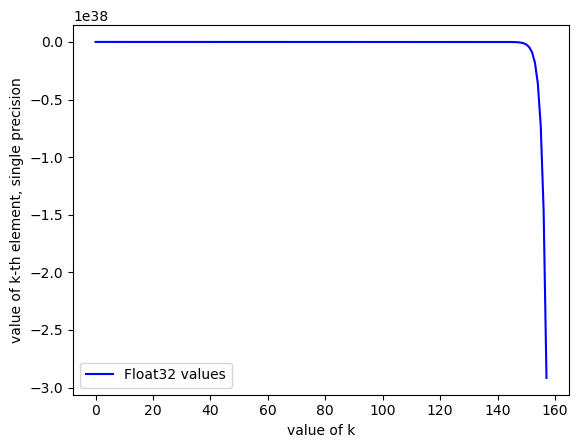
\includegraphics[width=0.67\textwidth]{img/float32-1.png}
	}
	\caption{Nieskalowany wykres wartości ciągu dla float32}
	\label{zad2:graph1}
\end{figure}
Widzimy, że po pewnym wyrazie ciągu (dokładniej po 9.), wszystkie wartości schodzą poniżej 0 i~ciąg jest stale malejący. Wyjaśnić to można poprzez zjawisko zwane 
\emph{underflow}~\cite{underflow_wiki}. W~pewnym momencie brakuje dokładności reprezentacji float32, żeby wystarczająco dokładnie zapisać wynik danego obliczenia i~wartość jest zaokrąglona 
do najbliższej możliwej - w tym przypadku okazuje się, że w~pewnym momencie jest nią liczba mniejsza od 0 w~reprezentacji float32.
\newline
\textbf{Uwaga!} Dla $k > 157$ wartości są tak małe, że wynik obliczenia jest nieokreślony ($-\infty$, dla $k > 159$ jest to nan). Zatem na powyższym wykresie nie są one obecne.

\newpage
Dla porównania przedstawiamy wykres, gdy nie używamy funkcji \emph{np.float32} na współczynnikach ciągu i~dostajemy bardziej sensowny, przypominający float64 wykres.
\begin{figure}[ht!]
	\centering{
		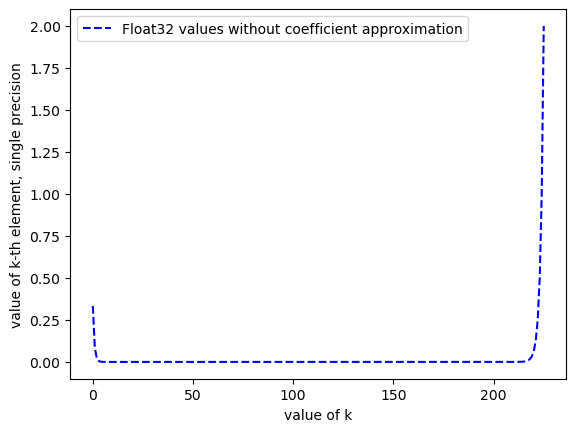
\includegraphics[width=0.67\textwidth]{img/float32-coeff.png}
	}
	\caption{Nieskalowany wykres wartości ciągu dla float32 bez przybliżenia współczynników}
	\label{zad2:graph2}
\end{figure}

Moglibyśmy wykorzystać ten sposób do obliczenia wyrazów ciągu, ale wtedy okazuje się, że float32 jest bardziej dokładny od float64 (w~dalszych testach błędu względnego float32 miałoby mniejszy błąd). Uznajemy to za niezbyt sensowne i~postanowiliśmy testować wszystkie funkcje, wykorzystując przybliżenie współczynników ciągu - nie patrzymy na to, że float32 ucieka do~$-\infty$, a~float64 do~$+\infty$. 

Poniżej przedstawiony jest wykres logarytmiczny wartości bezwzględnej wyrazów ciągu w~reprezentacji float32 (wykorzystujemy wartość bezwzględną dla wygody porównania wykresów z~ciągiem float64 w~przyszłości).
\begin{figure}[ht!]
	\centering{
		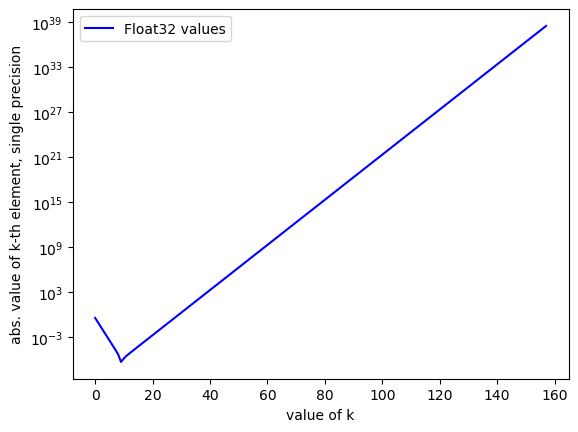
\includegraphics[width=0.67\textwidth]{img/float32-2.png}
	}
	\caption{Wykres symlog wartości ciągu dla float32}
	\label{zad2:graph3}
\end{figure}

\newpage
Poniżej prezentujemy logarytmiczny wykres wartości ciągu dla reprezentacji float64. 
\begin{figure}[ht!]
	\centering{
		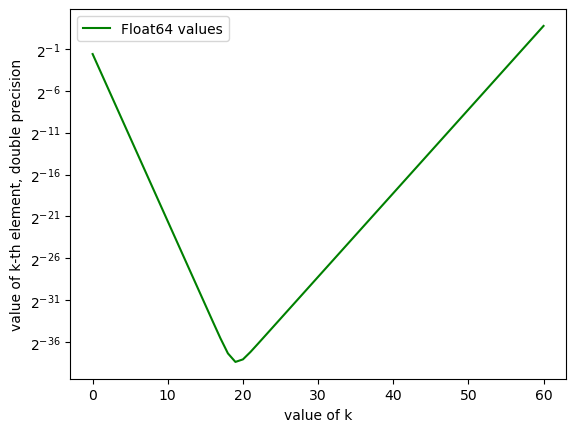
\includegraphics[width=0.67\textwidth]{img/float64.png}
	}
	\caption{Logarytmiczny wykres wartości ciągu dla float64}
	\label{zad2:graph4}
\end{figure}

Jak widać, podobnie do float32 (w~drugim rozważanym przypadku), float64 w~pewnym momencie osiąga minimum i~zaczyna rosnąć. Znowu związane to jest z~tym, że w~pewnym momencie 
następuje underflow, brakuje precyzji reprezentacji float64, żeby dokładnie przedstawić liczbę i~wykorzystywane są przybliżenia. Z~czasem coraz większa ilość przybliżeń się sumuje i~dostajemy wyrazy coraz bardziej różniące się od 
wartości rzeczywistej. W~pewnym momencie błąd reprezentacji powoduje, że wartość $x_k$ jest większa od $x_{k-1}$ i~wtedy ciąg rośnie w~nieskończoność.
\newline
\newline
Teraz spójrzmy na wykres dla reprezentacji z~biblioteki fractions.
\begin{figure}[ht!]
	\centering{
		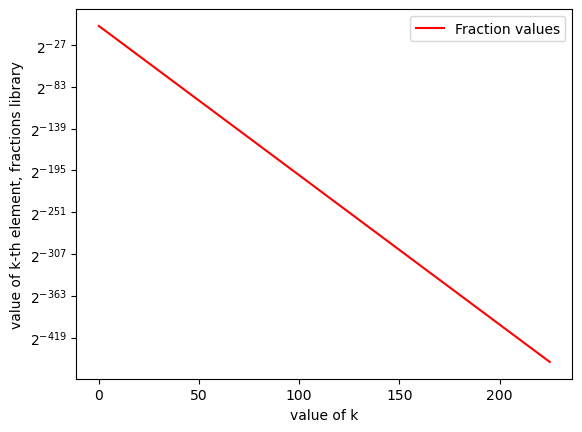
\includegraphics[width=0.67\textwidth]{img/fractions.png}
	}
	\caption{Logarytmiczny wykres wartości ciągu dla fractions}
	\label{zad2:graph5}
\end{figure}

Widać, że to jest najbardziej dokładna prezentacja. Ciąg wartości jest malejący i~większy od zera oraz reprezentuje dokładnie wartości wyliczone z~postaci jawnej ciągu (zobaczymy to poniżej, przy opracowaniu błędów względnych). Prawdopodobnie związane to jest z~tym, że postać jawna ciągu to 
$x_k = \frac{4^{-k}}{3}$, czyli każdy wyraz ciągu da się przedstawić dokładnie w~postaci ułamka i~patrząc na to, co Fractions robi pod spodem (mnoży, ewentualnie dodaje mianowniki i~liczniki, a~potem skraca ułamek), to taką dokładność można łatwo uzasadnić tym, że w~każdym momencie działamy na liczbach całkowitych (mianowniku i~liczniku). Dla naszego przypadku, kiedy wyrazy ciągu są wymierne i~w~dodatku do tego łatwo znaleźć k-ty wyraz w~postaci ułamka, Fraction jest najbardziej sensowną reprezentacją.

Poniżej przedstawiamy porównanie wszystkich wyników. Zauważamy między innymi, że rzeczywiste wartości ciągu w~zasadzie nakładają się na wykres wartości uzyskanych z~Fraction.
\begin{figure}[ht!]
	\centering{
		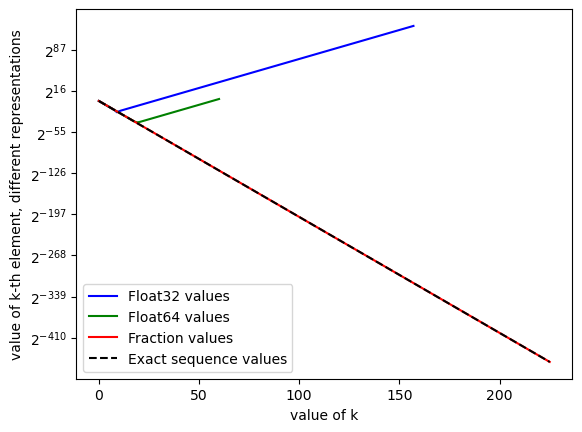
\includegraphics[width=0.67\textwidth]{img/all-values.png}
	}
	\caption{Wykres wspólny wartości ciągu dla różnych precyzji}
	\label{zad2:graph6}
\end{figure}

\subsection{Błędy względne}
\quad Przechodząc teraz do opracowania błędów względnych naszych reprezentacji, zaczniemy znów od float32.
\begin{figure}[h!]
	\centering{
		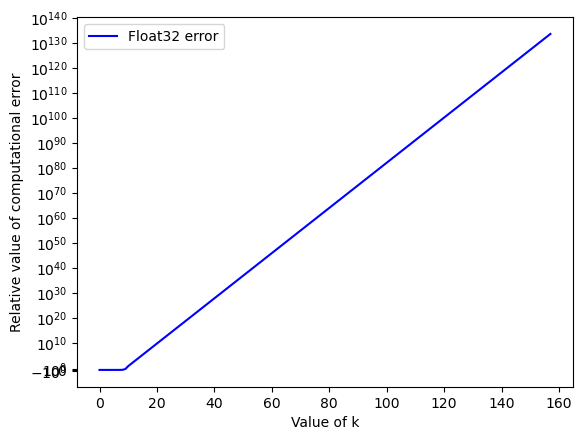
\includegraphics[width=0.67\textwidth]{img/float32-err.png}
	}
	\caption{Logarytmiczny wykres błędu względnego wyrazów ciągu dla float32}
	\label{zad2:graph7}
\end{figure}

Tak jak przewidywaliśmy przy wyjaśnieniu zachowania wykresów float32 i~float64, do pewnego momentu obliczenia są zapisywane w~miarę dokładnie, ale po jakimś czasie ograniczona precyzja powoduje underflow i~błąd zaczyna rosnąć eksponencjalnie (wykres jest w~skali logarytmicznej). Można zatem stwierdzić, że reprezentacja float32 dla naszego ciągu była dokładna tylko dla pierwszych 10 wyrazów.

Podobną analizę przeprowadzamy dla reprezentacji float64.
\begin{figure}[h!]
	\centering{
		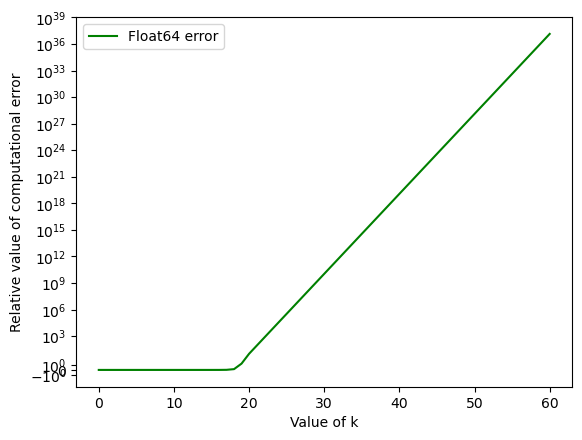
\includegraphics[width=0.67\textwidth]{img/float64-err.png}
	}
	\caption{Logarytmiczny wykres błędu względnego wyrazów ciągu dla float64}
	\label{zad2:graph8}
\end{figure}

Widzimy podobną do float32 sytuację - do pewnego momentu nasze obliczenia mają dużą precyzję, ale po tym, jak dochodzimy do momentu, gdy wiele underflow z rzędu powoduje zmniejszenie precyzji, błąd rośnie bardzo szybko.

Fractions wyróżnia się spośród badanych reprezentacji swoim zerowym błędem.
\begin{figure}[h!]
	\centering{
		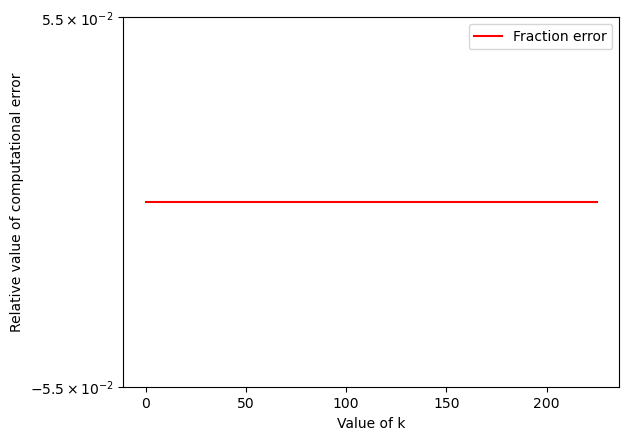
\includegraphics[width=0.67\textwidth]{img/fractions-err.png}
	}
	\caption{Logarytmiczny wykres błędu względnego wyrazów ciągu dla fractions}
	\label{zad2:graph9}
\end{figure}

Ponownie nasze spostrzeżenia odnośnie dobrej precyzji fractions w tym zadaniu (między innymi ze względu na to, że wyraz ogólny ciągu da się w~prosty sposób opisać za pomocą odpowiedniego ułamka) się sprawdzają. 

\newpage
Podsumujmy nasze rozważania, przedstawiając wspólny wykres wszystkich błędów względnych.
\begin{figure}[h!]
	\centering{
		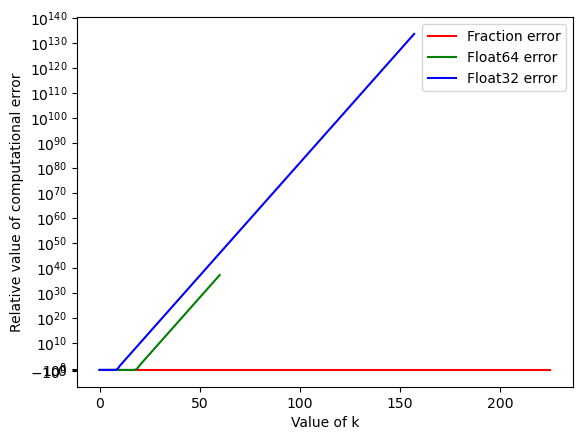
\includegraphics[width=0.67\textwidth]{img/all-err.png}
	}
	\caption{Logarytmiczny wykres błędu względnego wyrazów ciągu dla wszystkich precyzji}
	\label{zad2:graph10}
\end{figure}

Na tym wykresie widzimy, na ile floaty zachowują się w~podobny sposób. Poniżej na kolejnym wykresie lepiej widać 
moment, gdy każdy z~floatów zaczyna szybko tracić precyzję.

\begin{figure}[h!]
	\centering{
		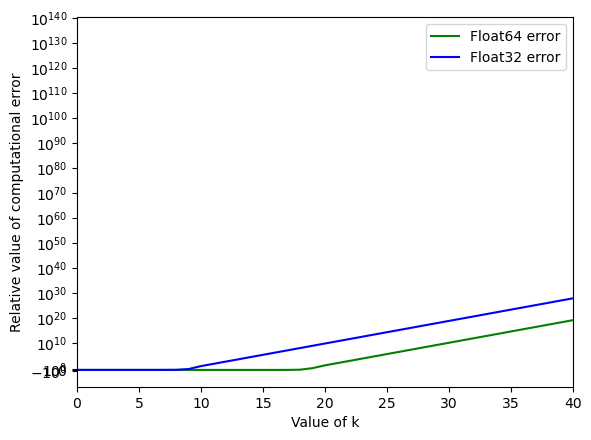
\includegraphics[width=0.67\textwidth]{img/float64-32-err.png}
	}
	\caption{Porównanie wartości błędu względnego dla float32 i~float64}
	\label{zad2:graph11}
\end{figure}

Z opracowania danych wynika, że float32 osiąga swoje minimum dla 9. wyrazu, a float64 dla 19. wyrazu. To jest mniej więcej zgodne z~przedstawieniem tego, jaką precyzję ma każda z~tych reprezentacji, gdyż float64 używa dwa razy więcej bitów i~wartość minimalna jest rzędu $10^{-12}$, a~w~przypadku float32 jest to tylko $10^{-7}$ (dla porównania, najmniejszy wyraz ciągu obliczonego za pomocą fractions to około $10^{-136}$). Ciekawym i~może trochę kontrintuicyjnym spostrzeżeniem jest to, że zarówno błędy względne float32, jak i~float64, mają podobne tempo wzrostu po momencie, kiedy zaczynają gwałtownie rosnąć.

\newpage  


\section{Podsumowanie}

\quad W ramach tego laboratorium przeprowadziliśmy analizę numerycznych metod obliczania pochodnej funkcji i~wyrazów ciągu rekurencyjnego oraz dokonaliśmy analizy błędów związanych z~tymi metodami.

W pierwszym zadaniu zaimplementowaliśmy numeryczną metodę obliczania pochodnej funkcji, używając przybliżenia za pomocą ilorazu różnicowego. Przetestowaliśmy tę metodę dla funkcji tangens oraz wyznaczyliśmy błąd, porównując wyniki numeryczne z~prawdziwą wartością pochodnej. Następnie przedstawiliśmy wykresy wartości bezwzględnej błędu metody, błędu numerycznego oraz błędu obliczeniowego w zależności od kroku $h$. Zauważyliśmy, że błąd obliczeniowy osiąga minimum dla określonej wartości $h$, co zgadza się z teoretycznymi przewidywaniami, jakie wynikają z analizy 
błędów numerycznych.

W drugim zadaniu zaimplementowaliśmy program generujący wyrazy ciągu zdefiniowanego równaniem różnicowym. Przeprowadziliśmy obliczenia dla różnych precyzji (pojedynczej, podwójnej oraz reprezentacji ułamków) i~narysowaliśmy wykresy wartości ciągu w~zależności od $k$. Dodatkowo, przedstawiliśmy wykres wartości bezwględnej błędu względnego w~zależności od $k$. 
Zaobserwowaliśmy, że wartości ciągu stale maleją wraz ze wzrostem $k$~jedynie dla reprezentacji fractions, a float32 i~float64 zachowują precyzję tylko dla ograniczonej ilości początkowych wyrazów.


\begin{thebibliography}{3}

\bibitem{teams_materials}
Materiały pomocnicze do laboratorium zamieszczone na platformie Teams w~katalogu \emph{lab01/lab1-intro.pdf}.


\bibitem{underflow_wiki}
Artykuł o `Arithmetic underflow` z wikipedii \url{https://en.wikipedia.org/wiki/Arithmetic_underflow}.

\end{thebibliography}

\end{document}
